\subsection{Atollic TrueSTUDIO}

\begin{figure}[ht]
	\centering
	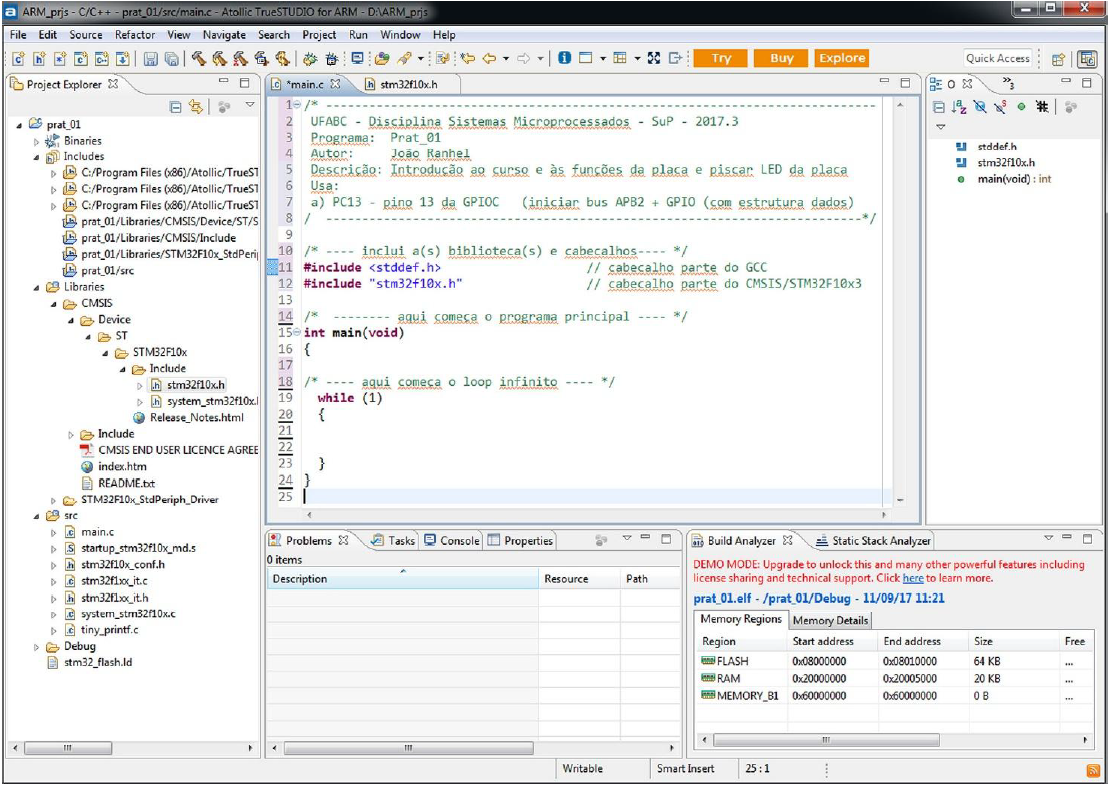
\includegraphics[width=0.8\textwidth]{figures/atollic}
	\caption{Interface Atollic \cite{apostila_microprossados}}
\end{figure}

A IDE a ser usada para programar um STM32 seria o TrueSTUDIO, distribuído pela
Atollic, que foi adquirida pela STMicroelectronics em 2017. Trata-se de um
software livre para programar em C/C++, criado com base na plataforma Eclipse,
e que possui todas as funções esperadas para o trabalho com o STM32, tais como
edição, compilação e debugging. Uma de seus principais vantagens é não haver
limites para tamanho de projeto, o que o torna ideal para trabalhos
profissionais. O TrueSTUDIO deixou de receber atualizações em 2017,
depois da aquisição pela STMicroelectronics.\cite{apostila_microprossados}



\subsection{Arduino}
Devido a complicações nas configurações de múltiplas saídas de PWM com o
TrueSTUDIO, optou-se por usar Arduino como alternativa. Um obstáculo a essa
alternativa é que o Arduino não é compatível com STM32 nativamente, porém um
o projeto STM32duino \cite{STM32duino}, criado por Frédéric Pillon, engenheiro
de software na STMicroelectronics \cite{fpistm}, permite instalar a bibliotecas
do STM32 no Arduino. No momento de escrita deste trabalho, o projeto era
compatível apenas com a versão 1.8 da IDE do Arduino.

\begin{figure}[ht]
	\centering
	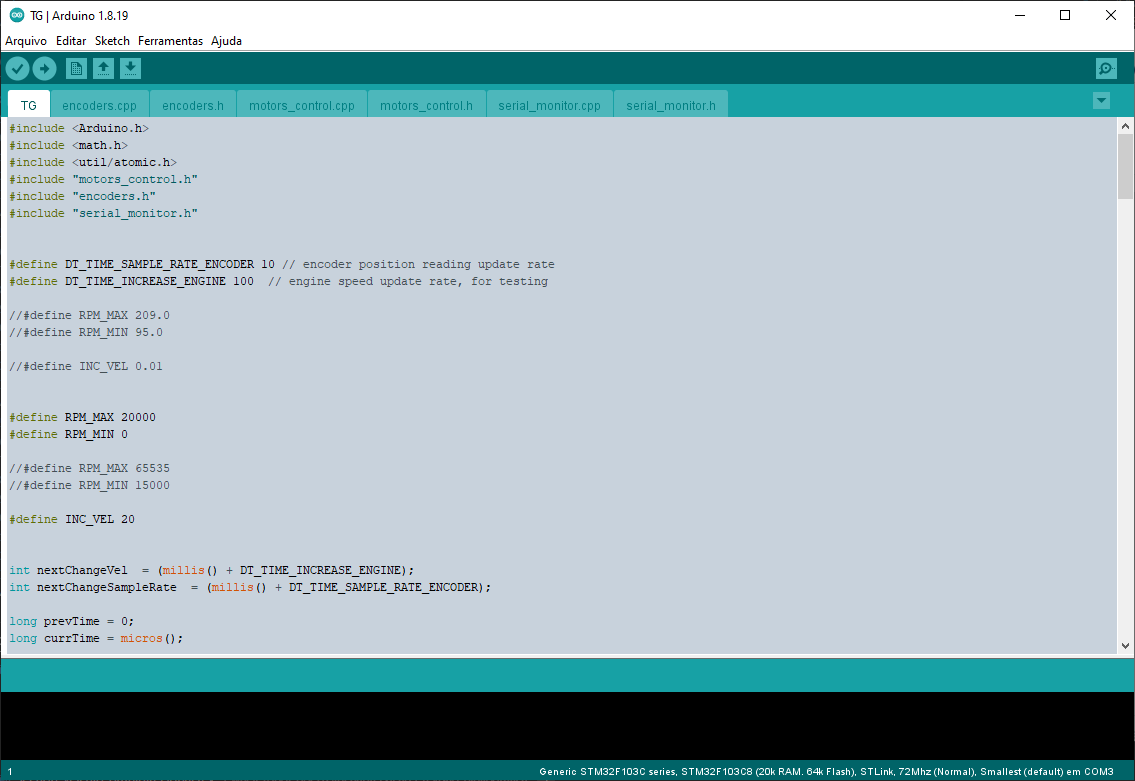
\includegraphics[width=1\textwidth]{figures/arduino}
	\caption{Interface Arduino}
\end{figure}



